%%%%%%%%%%%%%%%%%%%%%%% file template.tex %%%%%%%%%%%%%%%%%%%%%%%%%
%
% This is a template file for the global option of the SVJour class
%
% Copy it to a new file with a new name and use it as the basis
% for your article
%
%%%%%%%%%%%%%%%%%%%%%%%% Springer-Verlag %%%%%%%%%%%%%%%%%%%%%%%%%%
%
% First comes an example EPS file -- just ignore it and
% proceed on the \documentclass line
\begin{filecontents*}{example.eps}
%!PS-Adobe-3.0 EPSF-3.0
%%BoundingBox: 19 19 221 221
%%CreationDate: Mon Sep 29 1997
%%Creator: programmed by hand (JK)
%%EndComments
gsave
newpath
  20 20 moveto
  20 220 lineto
  220 220 lineto
  220 20 lineto
closepath
2 setlinewidth
gsave
  .4 setgray fill
grestore
stroke
grestore
\end{filecontents*}
%
% Choose either the first of the next two \documentclass lines for one
% column journals or the second for two column journals.
%\documentclass[global,referee]{svjour}
%\documentclass[global,twocolumn,referee]{svjour}
\documentclass[global,twocolumn]{svjour}
% Remove option referee for final version
%
% Remove any % below to load the required packages
%\usepackage{latexsym}
%\usepackage{graphics}
\usepackage{graphicx}

% etc
%
% Insert the name of "your" journal with the command below:
\journalname{myjournal}
%
\begin{document}
%
\title{Incremental Lazy View Regeneration for Complex Model Exploration}
%\subtitle{Do you have a subtitle?\\ If so, write it here}
\author{First author\inst{1} \and Second author\inst{2}% etc
% \thanks is optional - remove next line if not needed
\thanks{\emph{Present address:} Insert the address here if needed}%
}                     % Do not remove
%
\offprints{}          % Insert a name or remove this line
%
\institute{Insert the first address here \and the second here}
%
\date{Received: date / Revised version: date}
% The correct dates will be entered by the editor
%
\maketitle
%
\begin{abstract}
Insert your abstract here.
\end{abstract}
%
\section{Introduction}
\label{introduction}
Your text comes here. Separate text sections with


\section{Architecture}
\label{architecture}

\begin{figure*}
	\centering
	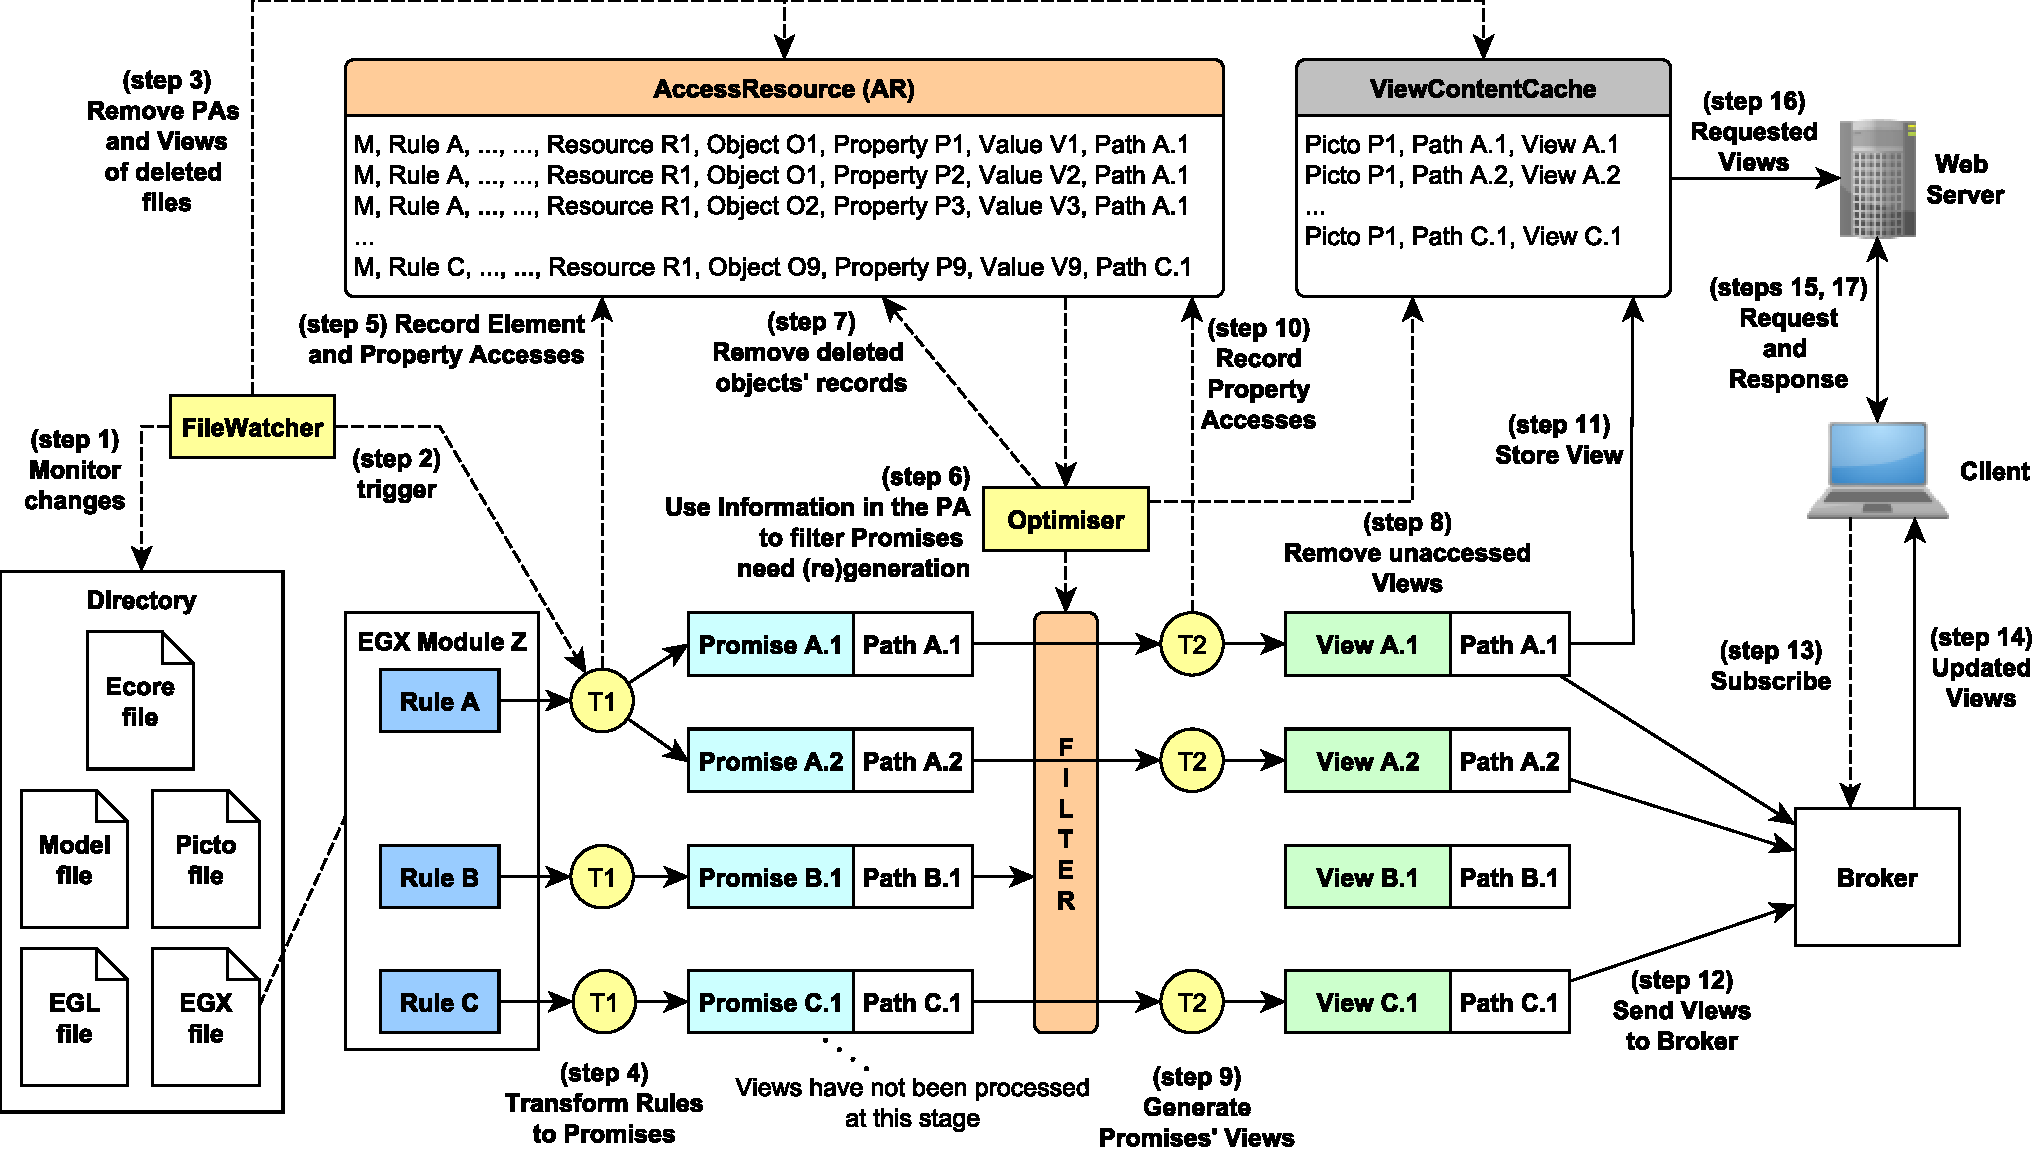
\includegraphics[width=\linewidth]{figures/architecture.pdf}
	\caption{The architecture of Picto Web for incremental lazy view regeneration.}
	\label{fig:architecture} 
\end{figure*}

The incremental regeneration of Picto Web's views follows the steps in Figure \ref{fig:architecture}. 

Picto Web has a singleton called \textsf{FileWatcher} that is responsible for monitoring changes on model files in a working directory, including creating and deleting a file (step 1). Every change to a file -- when the file is saved -- will trigger Picto Web to load the associate model transformation (EGX) file and other required files (e.g., the related template, model, metamodel files) into the memory and perform transformation \textsf{T1} (step 2). If the change is the deletion of a file, the \textsf{FileWatcher} will remove all related access records and view cache associated with the file (step 3).

Picto Web adopts the lazy transformation approach. The text generation in EGX/EGL commonly takes rules and templates as its inputs. When executed, the generation immediately processes them to produce the output files. However, in the lazy approach, only the rules are processed immediately to produce promises (step 4). Promises are the entities that will be transformed into views later in step 9. In other words, a promise only holds a reference to the template, but the template has not been processed yet to generate the target file. Every rule can produce more than one promise, and every promise is associated with a view, and it uses the path of the view in the tree view as its identifier. 

When performing the generation of promises in step 4, Picto Web records accesses to model elements and their properties and stores the accesses to the \textsf{AccessResource} (step 5). The \textsf{Optimiser} collects all the necessary information from the access resource and uses it to optimise the regeneration of views. In step 6, the \textsf{Optimiser} filters the promises and only selects them that will produce views affected by the changes applied to the files in step 1. Moreover, using the information in the \textsf{AccessResource}, the \textsf{Optimiser} also removes access records in the \textsf{AccessResource} and views in the \textsf{ViewContentCache} that are associated with elements that has been deleted to free memory space (steps 7 and 8). 

Similar to step 5, when the transformation \textsf{T2} processes the templates of the filtered promises to generate the target views, Picto Web also records element and property accesses and stores them to the \textsf{AccessResource} (step 10). Not all views are generated since the promises have been filtered by the \textsf{Optimiser}. After that, the generated new views are the store into the \textsf{ViewContentCache} (step 11). The new views also are sent to the \textsf{Broker} -- a broker server --  to be retrieved later by clients (step 12).

A client that accesses Picto Web using a web browser automatically subscribes to the \textsf{Broker} (step 13). Therefore, it retrieves the updated views immediately once a model file is changed, giving users a live visualisation experience of model editing (step 14). Also, the client can retrieve a specific view by sending a request to the web server (step 15). The web server then retrieves the requested view from the \textsf{ViewContentCache} (step 16) and sends it back to the client as a response (step 17).








%\section{Section title}
%\label{sec:1}
%and \cite{RefJ}
%\subsection{Subsection title}
%\label{sec:2}
%as required. Don't forget to give each section
%and subsection a unique label (see Sect.~\ref{sec:1}).
%%
%% For one-column wide figures use
%\begin{figure}
%% Use the relevant command for your figure-insertion program
%% to insert the figure file.
%% For example, with the option graphics use
%\resizebox{0.75\textwidth}{!}{%
%  
\includegraphics{example.eps}
%}
%% If not, use
%%\vspace{5cm}       % Give the correct figure height in cm
%\caption{Please write your figure caption here}
%\label{fig:1}       % Give a unique label
%\end{figure}
%%
%% For two-column wide figures use
%\begin{figure*}
%% Use the relevant command for your figure-insertion program
%% to insert the figure file. See example above.
%% If not, use
%\vspace*{5cm}       % Give the correct figure height in cm
%\caption{Please write your figure caption here}
%\label{fig:2}       % Give a unique label
%\end{figure*}
%%
%% For tables use
%\begin{table}
%\caption{Please write your table caption here}
%\label{tab:1}       % Give a unique label
%% For LaTeX tables use
%\begin{tabular}{lll}
%\hline\noalign{\smallskip}
%first & second & third  \\
%\noalign{\smallskip}\hline\noalign{\smallskip}
%number & number & number \\
%number & number & number \\
%\noalign{\smallskip}\hline
%\end{tabular}
%% Or use
%\vspace*{5cm}  % with the correct table height
%\end{table}
%%
%% BibTeX users please use
%% \bibliographystyle{}
%% \bibliography{}
%%
%% Non-BibTeX users please use
%\begin{thebibliography}{}
%%
%% and use \bibitem to create references.
%%
%\bibitem{RefJ}
%% Format for Journal Reference
%Author, Journal \textbf{Volume,} (year) page numbers.
%% Format for books
%\bibitem{RefB}
%Author, \textit{Book title} (Publisher, place year) page numbers
%% etc
%\end{thebibliography}


\end{document}

% end of file template.tex

